% This file was created by matlab2tikz.
%
%The latest updates can be retrieved from
%  http://www.mathworks.com/matlabcentral/fileexchange/22022-matlab2tikz-matlab2tikz
%where you can also make suggestions and rate matlab2tikz.
%
\definecolor{mycolor1}{rgb}{0.00000,0.44700,0.74100}%
\definecolor{mycolor2}{rgb}{0.85000,0.32500,0.09800}%
%
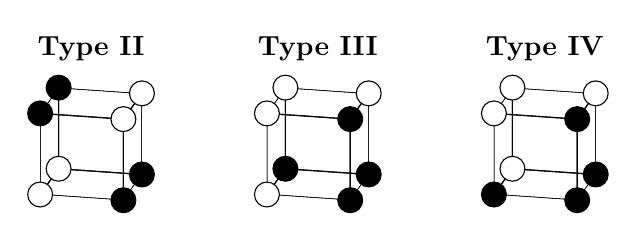
\begin{tikzpicture}

\begin{axis}[%
width=0.509in,
height=0.563in,
at={(0.347in,0.265in)},
scale only axis,
plot box ratio=1 1 1,
xmin=-1,
xmax=1,
tick align=outside,
ymin=-1,
ymax=1,
zmin=-1,
zmax=1,
view={-77.4711922908485}{18.0246645268103},
hide axis,
title style={font=\bfseries},
title={Type II}
]

\addplot3[area legend,solid,draw=black,fill=blue,fill opacity=0,forget plot]
table[row sep=crcr] {%
x	y	z\\
-1	-1	-1\\
1	-1	-1\\
1	-1	1\\
-1	-1	1\\
}--cycle;

\addplot3[area legend,solid,draw=black,fill=blue,fill opacity=0,forget plot]
table[row sep=crcr] {%
x	y	z\\
1	-1	-1\\
1	1	-1\\
1	1	1\\
1	-1	1\\
}--cycle;

\addplot3[area legend,solid,draw=black,fill=blue,fill opacity=0,forget plot]
table[row sep=crcr] {%
x	y	z\\
1	1	-1\\
-1	1	-1\\
-1	1	1\\
1	1	1\\
}--cycle;

\addplot3[area legend,solid,draw=black,fill=blue,fill opacity=0,forget plot]
table[row sep=crcr] {%
x	y	z\\
-1	1	-1\\
-1	-1	-1\\
-1	-1	1\\
-1	1	1\\
}--cycle;

\addplot3[area legend,solid,draw=black,fill=blue,fill opacity=0,forget plot]
table[row sep=crcr] {%
x	y	z\\
-1	-1	-1\\
1	-1	-1\\
1	1	-1\\
-1	1	-1\\
}--cycle;

\addplot3[area legend,solid,draw=black,fill=blue,fill opacity=0,forget plot]
table[row sep=crcr] {%
x	y	z\\
-1	-1	1\\
1	-1	1\\
1	1	1\\
-1	1	1\\
}--cycle;
\addplot3 [color=mycolor1,mark size=4.5pt,only marks,mark=*,mark options={solid,fill=black,draw=black}]
 table[row sep=crcr] {%
-1	-1	-1\\
1	-1	-1\\
-1	1	1\\
1	1	1\\
};
 \node[align=center, text=white]
at (axis cs:-1,-1,-1) {A};
\node[align=center, text=white]
at (axis cs:1,-1,-1) {A};
\node[align=center, text=white]
at (axis cs:-1,1,1) {A};
\node[align=center, text=white]
at (axis cs:1,1,1) {A};
\addplot3 [color=mycolor2,mark size=4.5pt,only marks,mark=*,mark options={solid,fill=white,draw=black}]
 table[row sep=crcr] {%
-1	1	-1\\
1	1	-1\\
-1	-1	1\\
1	-1	1\\
};
 \node[align=center, text=black]
at (axis cs:-1,1,-1) {B};
\node[align=center, text=black]
at (axis cs:1,1,-1) {B};
\node[align=center, text=black]
at (axis cs:-1,-1,1) {B};
\node[align=center, text=black]
at (axis cs:1,-1,1) {B};
\end{axis}

\begin{axis}[%
width=0.509in,
height=0.563in,
at={(1.481in,0.265in)},
scale only axis,
plot box ratio=1 1 1,
xmin=-1,
xmax=1,
tick align=outside,
ymin=-1,
ymax=1,
zmin=-1,
zmax=1,
view={-77.4711922908485}{18.0246645268103},
hide axis,
title style={font=\bfseries},
title={Type III}
]

\addplot3[area legend,solid,draw=black,fill=blue,fill opacity=0,forget plot]
table[row sep=crcr] {%
x	y	z\\
-1	-1	-1\\
1	-1	-1\\
1	-1	1\\
-1	-1	1\\
}--cycle;

\addplot3[area legend,solid,draw=black,fill=blue,fill opacity=0,forget plot]
table[row sep=crcr] {%
x	y	z\\
1	-1	-1\\
1	1	-1\\
1	1	1\\
1	-1	1\\
}--cycle;

\addplot3[area legend,solid,draw=black,fill=blue,fill opacity=0,forget plot]
table[row sep=crcr] {%
x	y	z\\
1	1	-1\\
-1	1	-1\\
-1	1	1\\
1	1	1\\
}--cycle;

\addplot3[area legend,solid,draw=black,fill=blue,fill opacity=0,forget plot]
table[row sep=crcr] {%
x	y	z\\
-1	1	-1\\
-1	-1	-1\\
-1	-1	1\\
-1	1	1\\
}--cycle;

\addplot3[area legend,solid,draw=black,fill=blue,fill opacity=0,forget plot]
table[row sep=crcr] {%
x	y	z\\
-1	-1	-1\\
1	-1	-1\\
1	1	-1\\
-1	1	-1\\
}--cycle;

\addplot3[area legend,solid,draw=black,fill=blue,fill opacity=0,forget plot]
table[row sep=crcr] {%
x	y	z\\
-1	-1	1\\
1	-1	1\\
1	1	1\\
-1	1	1\\
}--cycle;
\addplot3 [color=mycolor1,mark size=4.5pt,only marks,mark=*,mark options={solid,fill=black,draw=black}]
 table[row sep=crcr] {%
-1	-1	-1\\
1	-1	-1\\
1	1	-1\\
-1	-1	1\\
};
 \node[align=center, text=white]
at (axis cs:-1,-1,-1) {A};
\node[align=center, text=white]
at (axis cs:1,-1,-1) {A};
\node[align=center, text=white]
at (axis cs:1,1,-1) {A};
\node[align=center, text=white]
at (axis cs:-1,-1,1) {A};
\addplot3 [color=mycolor2,mark size=4.5pt,only marks,mark=*,mark options={solid,fill=white,draw=black}]
 table[row sep=crcr] {%
-1	1	-1\\
1	-1	1\\
-1	1	1\\
1	1	1\\
};
 \node[align=center, text=black]
at (axis cs:-1,1,-1) {B};
\node[align=center, text=black]
at (axis cs:1,-1,1) {B};
\node[align=center, text=black]
at (axis cs:-1,1,1) {B};
\node[align=center, text=black]
at (axis cs:1,1,1) {B};
\end{axis}

\begin{axis}[%
width=0.509in,
height=0.563in,
at={(2.616in,0.265in)},
scale only axis,
plot box ratio=1 1 1,
xmin=-1,
xmax=1,
tick align=outside,
ymin=-1,
ymax=1,
zmin=-1,
zmax=1,
view={-77.4711922908485}{18.0246645268103},
hide axis,
title style={font=\bfseries},
title={Type IV}
]

\addplot3[area legend,solid,draw=black,fill=blue,fill opacity=0,forget plot]
table[row sep=crcr] {%
x	y	z\\
-1	-1	-1\\
1	-1	-1\\
1	-1	1\\
-1	-1	1\\
}--cycle;

\addplot3[area legend,solid,draw=black,fill=blue,fill opacity=0,forget plot]
table[row sep=crcr] {%
x	y	z\\
1	-1	-1\\
1	1	-1\\
1	1	1\\
1	-1	1\\
}--cycle;

\addplot3[area legend,solid,draw=black,fill=blue,fill opacity=0,forget plot]
table[row sep=crcr] {%
x	y	z\\
1	1	-1\\
-1	1	-1\\
-1	1	1\\
1	1	1\\
}--cycle;

\addplot3[area legend,solid,draw=black,fill=blue,fill opacity=0,forget plot]
table[row sep=crcr] {%
x	y	z\\
-1	1	-1\\
-1	-1	-1\\
-1	-1	1\\
-1	1	1\\
}--cycle;

\addplot3[area legend,solid,draw=black,fill=blue,fill opacity=0,forget plot]
table[row sep=crcr] {%
x	y	z\\
-1	-1	-1\\
1	-1	-1\\
1	1	-1\\
-1	1	-1\\
}--cycle;

\addplot3[area legend,solid,draw=black,fill=blue,fill opacity=0,forget plot]
table[row sep=crcr] {%
x	y	z\\
-1	-1	1\\
1	-1	1\\
1	1	1\\
-1	1	1\\
}--cycle;
\addplot3 [color=mycolor1,mark size=4.5pt,only marks,mark=*,mark options={solid,fill=black,draw=black}]
 table[row sep=crcr] {%
-1	-1	-1\\
1	-1	-1\\
-1	1	-1\\
-1	-1	1\\
};
 \node[align=center, text=white]
at (axis cs:-1,-1,-1) {A};
\node[align=center, text=white]
at (axis cs:1,-1,-1) {A};
\node[align=center, text=white]
at (axis cs:-1,1,-1) {A};
\node[align=center, text=white]
at (axis cs:-1,-1,1) {A};
\addplot3 [color=mycolor2,mark size=4.5pt,only marks,mark=*,mark options={solid,fill=white,draw=black}]
 table[row sep=crcr] {%
1	1	-1\\
1	-1	1\\
-1	1	1\\
1	1	1\\
};
 \node[align=center, text=black]
at (axis cs:1,1,-1) {B};
\node[align=center, text=black]
at (axis cs:1,-1,1) {B};
\node[align=center, text=black]
at (axis cs:-1,1,1) {B};
\node[align=center, text=black]
at (axis cs:1,1,1) {B};
\end{axis}
\end{tikzpicture}%